\documentclass{report}

\documentclass[12pt]{article}
\usepackage{array}
\usepackage{color}
\usepackage{amsthm}
\usepackage{eufrak}
\usepackage{lipsum}
\usepackage{pifont}
\usepackage{yfonts}
\usepackage{amsmath}
\usepackage{amssymb}
\usepackage{ccfonts}
\usepackage{comment} \usepackage{amsfonts}
\usepackage{fancyhdr}
\usepackage{graphicx}
\usepackage{listings}
\usepackage{mathrsfs}
\usepackage{setspace}
\usepackage{textcomp}
\usepackage{blindtext}
\usepackage{enumerate}
\usepackage{microtype}
\usepackage{xfakebold}
\usepackage{kantlipsum}
%\usepackage{draftwatermark}
\usepackage[spanish]{babel}
\usepackage[margin=1.5cm, top=2cm, bottom=2cm]{geometry}
\usepackage[framemethod=tikz]{mdframed}
\usepackage[colorlinks=true,citecolor=blue,linkcolor=red,urlcolor=magenta]{hyperref}

%//////////////////////////////////////////////////////
% Watermark configuration
%//////////////////////////////////////////////////////
%\SetWatermarkScale{4}
%\SetWatermarkColor{black}
%\SetWatermarkLightness{0.95}
%\SetWatermarkText{\texttt{Watermark}}

%//////////////////////////////////////////////////////
% Frame configuration
%//////////////////////////////////////////////////////
\newmdenv[tikzsetting={draw=gray,fill=white,fill opacity=0},backgroundcolor=none]{Frame}

%//////////////////////////////////////////////////////
% Font style configuration
%//////////////////////////////////////////////////////
\renewcommand{\familydefault}{\ttdefault}
\renewcommand{\rmdefault}{tt}

%//////////////////////////////////////////////////////
% Bold configuration
%//////////////////////////////////////////////////////
\newcommand{\fbseries}{\unskip\setBold\aftergroup\unsetBold\aftergroup\ignorespaces}
\makeatletter
\newcommand{\setBoldness}[1]{\def\fake@bold{#1}}
\makeatother

%//////////////////////////////////////////////////////
% Default font configuration
%//////////////////////////////////////////////////////
\DeclareFontFamily{\encodingdefault}{\ttdefault}{%
  \hyphenchar\font=\defaulthyphenchar
  \fontdimen2\font=0.33333em
  \fontdimen3\font=0.16667em
  \fontdimen4\font=0.11111em
  \fontdimen7\font=0.11111em}


%From M275 "Topology" at SJSU
\newcommand{\id}{\mathrm{id}}
\newcommand{\taking}[1]{\xrightarrow{#1}}
\newcommand{\inv}{^{-1}}

%From M170 "Introduction to Graph Theory" at SJSU
\DeclareMathOperator{\diam}{diam}
\DeclareMathOperator{\ord}{ord}
\newcommand{\defeq}{\overset{\mathrm{def}}{=}}

%From the USAMO .tex files
\newcommand{\ts}{\textsuperscript}
\newcommand{\dg}{^\circ}
\newcommand{\ii}{\item}

% % From Math 55 and Math 145 at Harvard
% \newenvironment{subproof}[1][Proof]{%
% \begin{proof}[#1] \renewcommand{\qedsymbol}{$\blacksquare$}}%
% {\end{proof}}

\newcommand{\liff}{\leftrightarrow}
\newcommand{\lthen}{\rightarrow}
\newcommand{\opname}{\operatorname}
\newcommand{\surjto}{\twoheadrightarrow}
\newcommand{\injto}{\hookrightarrow}
\newcommand{\On}{\mathrm{On}} % ordinals
\DeclareMathOperator{\img}{im} % Image
\DeclareMathOperator{\Img}{Im} % Image
\DeclareMathOperator{\coker}{coker} % Cokernel
\DeclareMathOperator{\Coker}{Coker} % Cokernel
\DeclareMathOperator{\Ker}{Ker} % Kernel
\DeclareMathOperator{\rank}{rank}
\DeclareMathOperator{\Spec}{Spec} % spectrum
\DeclareMathOperator{\Tr}{Tr} % trace
\DeclareMathOperator{\pr}{pr} % projection
\DeclareMathOperator{\ext}{ext} % extension
\DeclareMathOperator{\pred}{pred} % predecessor
\DeclareMathOperator{\dom}{dom} % domain
\DeclareMathOperator{\ran}{ran} % range
\DeclareMathOperator{\Hom}{Hom} % homomorphism
\DeclareMathOperator{\Mor}{Mor} % morphisms
\DeclareMathOperator{\End}{End} % endomorphism

\newcommand{\eps}{\epsilon}
\newcommand{\veps}{\varepsilon}
\newcommand{\ol}{\overline}
\newcommand{\ul}{\underline}
\newcommand{\wt}{\widetilde}
\newcommand{\wh}{\widehat}
\newcommand{\vocab}[1]{\textbf{\color{blue} #1}}
\providecommand{\half}{\frac{1}{2}}
\newcommand{\dang}{\measuredangle} %% Directed angle
\newcommand{\ray}[1]{\overrightarrow{#1}}
\newcommand{\seg}[1]{\overline{#1}}
\newcommand{\arc}[1]{\wideparen{#1}}
\DeclareMathOperator{\cis}{cis}
\DeclareMathOperator*{\lcm}{lcm}
\DeclareMathOperator*{\argmin}{arg min}
\DeclareMathOperator*{\argmax}{arg max}
\newcommand{\cycsum}{\sum_{\mathrm{cyc}}}
\newcommand{\symsum}{\sum_{\mathrm{sym}}}
\newcommand{\cycprod}{\prod_{\mathrm{cyc}}}
\newcommand{\symprod}{\prod_{\mathrm{sym}}}
\newcommand{\Qed}{\begin{flushright}\qed\end{flushright}}
\newcommand{\parinn}{\setlength{\parindent}{1cm}}
\newcommand{\parinf}{\setlength{\parindent}{0cm}}
% \newcommand{\norm}{\|\cdot\|}
\newcommand{\inorm}{\norm_{\infty}}
\newcommand{\opensets}{\{V_{\alpha}\}_{\alpha\in I}}
\newcommand{\oset}{V_{\alpha}}
\newcommand{\opset}[1]{V_{\alpha_{#1}}}
\newcommand{\lub}{\text{lub}}
\newcommand{\del}[2]{\frac{\partial #1}{\partial #2}}
\newcommand{\Del}[3]{\frac{\partial^{#1} #2}{\partial^{#1} #3}}
\newcommand{\deld}[2]{\dfrac{\partial #1}{\partial #2}}
\newcommand{\Deld}[3]{\dfrac{\partial^{#1} #2}{\partial^{#1} #3}}
\newcommand{\lm}{\lambda}
\newcommand{\uin}{\mathbin{\rotatebox[origin=c]{90}{$\in$}}}
\newcommand{\usubset}{\mathbin{\rotatebox[origin=c]{90}{$\subset$}}}
\newcommand{\lt}{\left}
\newcommand{\rt}{\right}
\newcommand{\paren}[1]{\left(#1\right)}
\newcommand{\bs}[1]{\boldsymbol{#1}}
\newcommand{\exs}{\exists}
\newcommand{\st}{\strut}
\newcommand{\dps}[1]{\displaystyle{#1}}

\newcommand{\sol}{\setlength{\parindent}{0cm}\textbf{\textit{Solution:}}\setlength{\parindent}{1cm} }
\newcommand{\solve}[1]{\setlength{\parindent}{0cm}\textbf{\textit{Solution: }}\setlength{\parindent}{1cm}#1 \Qed}

% Things Lie
\newcommand{\kb}{\mathfrak b}
\newcommand{\kg}{\mathfrak g}
\newcommand{\kh}{\mathfrak h}
\newcommand{\kn}{\mathfrak n}
\newcommand{\ku}{\mathfrak u}
\newcommand{\kz}{\mathfrak z}
\DeclareMathOperator{\Ext}{Ext} % Ext functor
\DeclareMathOperator{\Tor}{Tor} % Tor functor
\newcommand{\gl}{\opname{\mathfrak{gl}}} % frak gl group
\renewcommand{\sl}{\opname{\mathfrak{sl}}} % frak sl group chktex 6

% More script letters etc.
\newcommand{\SA}{\mathcal A}
\newcommand{\SB}{\mathcal B}
\newcommand{\SC}{\mathcal C}
\newcommand{\SF}{\mathcal F}
\newcommand{\SG}{\mathcal G}
\newcommand{\SH}{\mathcal H}
\newcommand{\OO}{\mathcal O}

\newcommand{\SCA}{\mathscr A}
\newcommand{\SCB}{\mathscr B}
\newcommand{\SCC}{\mathscr C}
\newcommand{\SCD}{\mathscr D}
\newcommand{\SCE}{\mathscr E}
\newcommand{\SCF}{\mathscr F}
\newcommand{\SCG}{\mathscr G}
\newcommand{\SCH}{\mathscr H}

% Mathfrak primes
\newcommand{\km}{\mathfrak m}
\newcommand{\kp}{\mathfrak p}
\newcommand{\kq}{\mathfrak q}

% number sets
\newcommand{\RR}[1][]{\ensuremath{\ifstrempty{#1}{\mathbb{R}}{\mathbb{R}^{#1}}}}
\newcommand{\NN}[1][]{\ensuremath{\ifstrempty{#1}{\mathbb{N}}{\mathbb{N}^{#1}}}}
\newcommand{\ZZ}[1][]{\ensuremath{\ifstrempty{#1}{\mathbb{Z}}{\mathbb{Z}^{#1}}}}
\newcommand{\QQ}[1][]{\ensuremath{\ifstrempty{#1}{\mathbb{Q}}{\mathbb{Q}^{#1}}}}
\newcommand{\CC}[1][]{\ensuremath{\ifstrempty{#1}{\mathbb{C}}{\mathbb{C}^{#1}}}}
\newcommand{\PP}[1][]{\ensuremath{\ifstrempty{#1}{\mathbb{P}}{\mathbb{P}^{#1}}}}
\newcommand{\HH}[1][]{\ensuremath{\ifstrempty{#1}{\mathbb{H}}{\mathbb{H}^{#1}}}}
\newcommand{\FF}[1][]{\ensuremath{\ifstrempty{#1}{\mathbb{F}}{\mathbb{F}^{#1}}}}
% expected value
\newcommand{\EE}{\ensuremath{\mathbb{E}}}
\newcommand{\charin}{\text{ char }}
\DeclareMathOperator{\sign}{sign}
\DeclareMathOperator{\Aut}{Aut}
\DeclareMathOperator{\Inn}{Inn}
\DeclareMathOperator{\Syl}{Syl}
\DeclareMathOperator{\Gal}{Gal}
\DeclareMathOperator{\GL}{GL} % General linear group
\DeclareMathOperator{\SL}{SL} % Special linear group

%---------------------------------------
% BlackBoard Math Fonts :-
%---------------------------------------

%Captital Letters
\newcommand{\bbA}{\mathbb{A}}	\newcommand{\bbB}{\mathbb{B}}
\newcommand{\bbC}{\mathbb{C}}	\newcommand{\bbD}{\mathbb{D}}
\newcommand{\bbE}{\mathbb{E}}	\newcommand{\bbF}{\mathbb{F}}
\newcommand{\bbG}{\mathbb{G}}	\newcommand{\bbH}{\mathbb{H}}
\newcommand{\bbI}{\mathbb{I}}	\newcommand{\bbJ}{\mathbb{J}}
\newcommand{\bbK}{\mathbb{K}}	\newcommand{\bbL}{\mathbb{L}}
\newcommand{\bbM}{\mathbb{M}}	\newcommand{\bbN}{\mathbb{N}}
\newcommand{\bbO}{\mathbb{O}}	\newcommand{\bbP}{\mathbb{P}}
\newcommand{\bbQ}{\mathbb{Q}}	\newcommand{\bbR}{\mathbb{R}}
\newcommand{\bbS}{\mathbb{S}}	\newcommand{\bbT}{\mathbb{T}}
\newcommand{\bbU}{\mathbb{U}}	\newcommand{\bbV}{\mathbb{V}}
\newcommand{\bbW}{\mathbb{W}}	\newcommand{\bbX}{\mathbb{X}}
\newcommand{\bbY}{\mathbb{Y}}	\newcommand{\bbZ}{\mathbb{Z}}

%---------------------------------------
% MathCal Fonts :-
%---------------------------------------

%Captital Letters
\newcommand{\mcA}{\mathcal{A}}	\newcommand{\mcB}{\mathcal{B}}
\newcommand{\mcC}{\mathcal{C}}	\newcommand{\mcD}{\mathcal{D}}
\newcommand{\mcE}{\mathcal{E}}	\newcommand{\mcF}{\mathcal{F}}
\newcommand{\mcG}{\mathcal{G}}	\newcommand{\mcH}{\mathcal{H}}
\newcommand{\mcI}{\mathcal{I}}	\newcommand{\mcJ}{\mathcal{J}}
\newcommand{\mcK}{\mathcal{K}}	\newcommand{\mcL}{\mathcal{L}}
\newcommand{\mcM}{\mathcal{M}}	\newcommand{\mcN}{\mathcal{N}}
\newcommand{\mcO}{\mathcal{O}}	\newcommand{\mcP}{\mathcal{P}}
\newcommand{\mcQ}{\mathcal{Q}}	\newcommand{\mcR}{\mathcal{R}}
\newcommand{\mcS}{\mathcal{S}}	\newcommand{\mcT}{\mathcal{T}}
\newcommand{\mcU}{\mathcal{U}}	\newcommand{\mcV}{\mathcal{V}}
\newcommand{\mcW}{\mathcal{W}}	\newcommand{\mcX}{\mathcal{X}}
\newcommand{\mcY}{\mathcal{Y}}	\newcommand{\mcZ}{\mathcal{Z}}


%---------------------------------------
% Bold Math Fonts :-
%---------------------------------------

%Captital Letters
\newcommand{\bmA}{\boldsymbol{A}}	\newcommand{\bmB}{\boldsymbol{B}}
\newcommand{\bmC}{\boldsymbol{C}}	\newcommand{\bmD}{\boldsymbol{D}}
\newcommand{\bmE}{\boldsymbol{E}}	\newcommand{\bmF}{\boldsymbol{F}}
\newcommand{\bmG}{\boldsymbol{G}}	\newcommand{\bmH}{\boldsymbol{H}}
\newcommand{\bmI}{\boldsymbol{I}}	\newcommand{\bmJ}{\boldsymbol{J}}
\newcommand{\bmK}{\boldsymbol{K}}	\newcommand{\bmL}{\boldsymbol{L}}
\newcommand{\bmM}{\boldsymbol{M}}	\newcommand{\bmN}{\boldsymbol{N}}
\newcommand{\bmO}{\boldsymbol{O}}	\newcommand{\bmP}{\boldsymbol{P}}
\newcommand{\bmQ}{\boldsymbol{Q}}	\newcommand{\bmR}{\boldsymbol{R}}
\newcommand{\bmS}{\boldsymbol{S}}	\newcommand{\bmT}{\boldsymbol{T}}
\newcommand{\bmU}{\boldsymbol{U}}	\newcommand{\bmV}{\boldsymbol{V}}
\newcommand{\bmW}{\boldsymbol{W}}	\newcommand{\bmX}{\boldsymbol{X}}
\newcommand{\bmY}{\boldsymbol{Y}}	\newcommand{\bmZ}{\boldsymbol{Z}}
%Small Letters
\newcommand{\bma}{\boldsymbol{a}}	\newcommand{\bmb}{\boldsymbol{b}}
\newcommand{\bmc}{\boldsymbol{c}}	\newcommand{\bmd}{\boldsymbol{d}}
\newcommand{\bme}{\boldsymbol{e}}	\newcommand{\bmf}{\boldsymbol{f}}
\newcommand{\bmg}{\boldsymbol{g}}	\newcommand{\bmh}{\boldsymbol{h}}
\newcommand{\bmi}{\boldsymbol{i}}	\newcommand{\bmj}{\boldsymbol{j}}
\newcommand{\bmk}{\boldsymbol{k}}	\newcommand{\bml}{\boldsymbol{l}}
\newcommand{\bmm}{\boldsymbol{m}}	\newcommand{\bmn}{\boldsymbol{n}}
\newcommand{\bmo}{\boldsymbol{o}}	\newcommand{\bmp}{\boldsymbol{p}}
\newcommand{\bmq}{\boldsymbol{q}}	\newcommand{\bmr}{\boldsymbol{r}}
\newcommand{\bms}{\boldsymbol{s}}	\newcommand{\bmt}{\boldsymbol{t}}
\newcommand{\bmu}{\boldsymbol{u}}	\newcommand{\bmv}{\boldsymbol{v}}
\newcommand{\bmw}{\boldsymbol{w}}	\newcommand{\bmx}{\boldsymbol{x}}
\newcommand{\bmy}{\boldsymbol{y}}	\newcommand{\bmz}{\boldsymbol{z}}

%---------------------------------------
% Scr Math Fonts :-
%---------------------------------------

\newcommand{\sA}{{\mathscr{A}}}   \newcommand{\sB}{{\mathscr{B}}}
\newcommand{\sC}{{\mathscr{C}}}   \newcommand{\sD}{{\mathscr{D}}}
\newcommand{\sE}{{\mathscr{E}}}   \newcommand{\sF}{{\mathscr{F}}}
\newcommand{\sG}{{\mathscr{G}}}   \newcommand{\sH}{{\mathscr{H}}}
\newcommand{\sI}{{\mathscr{I}}}   \newcommand{\sJ}{{\mathscr{J}}}
\newcommand{\sK}{{\mathscr{K}}}   \newcommand{\sL}{{\mathscr{L}}}
\newcommand{\sM}{{\mathscr{M}}}   \newcommand{\sN}{{\mathscr{N}}}
\newcommand{\sO}{{\mathscr{O}}}   \newcommand{\sP}{{\mathscr{P}}}
\newcommand{\sQ}{{\mathscr{Q}}}   \newcommand{\sR}{{\mathscr{R}}}
\newcommand{\sS}{{\mathscr{S}}}   \newcommand{\sT}{{\mathscr{T}}}
\newcommand{\sU}{{\mathscr{U}}}   \newcommand{\sV}{{\mathscr{V}}}
\newcommand{\sW}{{\mathscr{W}}}   \newcommand{\sX}{{\mathscr{X}}}
\newcommand{\sY}{{\mathscr{Y}}}   \newcommand{\sZ}{{\mathscr{Z}}}


%---------------------------------------
% Math Fraktur Font
%---------------------------------------

%Captital Letters
\newcommand{\mfA}{\mathfrak{A}}	\newcommand{\mfB}{\mathfrak{B}}
\newcommand{\mfC}{\mathfrak{C}}	\newcommand{\mfD}{\mathfrak{D}}
\newcommand{\mfE}{\mathfrak{E}}	\newcommand{\mfF}{\mathfrak{F}}
\newcommand{\mfG}{\mathfrak{G}}	\newcommand{\mfH}{\mathfrak{H}}
\newcommand{\mfI}{\mathfrak{I}}	\newcommand{\mfJ}{\mathfrak{J}}
\newcommand{\mfK}{\mathfrak{K}}	\newcommand{\mfL}{\mathfrak{L}}
\newcommand{\mfM}{\mathfrak{M}}	\newcommand{\mfN}{\mathfrak{N}}
\newcommand{\mfO}{\mathfrak{O}}	\newcommand{\mfP}{\mathfrak{P}}
\newcommand{\mfQ}{\mathfrak{Q}}	\newcommand{\mfR}{\mathfrak{R}}
\newcommand{\mfS}{\mathfrak{S}}	\newcommand{\mfT}{\mathfrak{T}}
\newcommand{\mfU}{\mathfrak{U}}	\newcommand{\mfV}{\mathfrak{V}}
\newcommand{\mfW}{\mathfrak{W}}	\newcommand{\mfX}{\mathfrak{X}}
\newcommand{\mfY}{\mathfrak{Y}}	\newcommand{\mfZ}{\mathfrak{Z}}
%Small Letters
\newcommand{\mfa}{\mathfrak{a}}	\newcommand{\mfb}{\mathfrak{b}}
\newcommand{\mfc}{\mathfrak{c}}	\newcommand{\mfd}{\mathfrak{d}}
\newcommand{\mfe}{\mathfrak{e}}	\newcommand{\mff}{\mathfrak{f}}
\newcommand{\mfg}{\mathfrak{g}}	\newcommand{\mfh}{\mathfrak{h}}
\newcommand{\mfi}{\mathfrak{i}}	\newcommand{\mfj}{\mathfrak{j}}
\newcommand{\mfk}{\mathfrak{k}}	\newcommand{\mfl}{\mathfrak{l}}
\newcommand{\mfm}{\mathfrak{m}}	\newcommand{\mfn}{\mathfrak{n}}
\newcommand{\mfo}{\mathfrak{o}}	\newcommand{\mfp}{\mathfrak{p}}
\newcommand{\mfq}{\mathfrak{q}}	\newcommand{\mfr}{\mathfrak{r}}
\newcommand{\mfs}{\mathfrak{s}}	\newcommand{\mft}{\mathfrak{t}}
\newcommand{\mfu}{\mathfrak{u}}	\newcommand{\mfv}{\mathfrak{v}}
\newcommand{\mfw}{\mathfrak{w}}	\newcommand{\mfx}{\mathfrak{x}}
\newcommand{\mfy}{\mathfrak{y}}	\newcommand{\mfz}{\mathfrak{z}}

\usepackage{float}
\usepackage{listing}

\title{\Huge{Mecánica}\\Tarea 4}
\author{\huge{Sergio Montoya Ramírez}}
\date{}

\begin{document}

\maketitle
\newpage% or \cleardoublepage
% \pdfbookmark[<level>]{<title>}{<dest>}
\pdfbookmark[section]{\contentsname}{toc}
\tableofcontents
\pagebreak

\chapter{}

\section{Enunciado}

Demuestre que $\epsilon^2=1+\frac{2EL^2}{mk^2}$

\section{Solución}

En este caso, tenemos que saber que $\varphi = 0$ y que la ecuación es $\frac{1}{r}=\frac{1+\varepsilon\cos\left( \varphi \right) }{P}$. Sin embargo tenemos que desarrollar primero la energia con
\begin{align*}
  E = \frac{L^2}{2mr^2}- \frac{k}{r}\\
  =\frac{1}{2r}\left( \frac{L^2}{mr}- 2k \right)
.\end{align*}

Ahora con esto queda:
\begin{align*}
  E &= \frac{1 + \varepsilon}{2P}\left( \frac{L^2\left( 1+\varepsilon \right) }{mp}-2k \right) \\
  &= \frac{\left( 1+\varepsilon \right)  mk}{2L^2}\left( k\left( 1 + \varepsilon \right)  - 2k \right)  \\
  &= \frac{mk}{2L^2}\left( k\left( \left( 1+\varepsilon \right)^2 - 2\left( 1 + \varepsilon \right)   \right)  \right)   \\
  &= \frac{mk^2}{2L^2}\left( 1 + 2\varepsilon + \varepsilon^2 - 2 - 2\varepsilon \right)  \\
  &= \frac{ mk^2}{2L^2}\left( \varepsilon^2-1 \right)  \\
  \frac{2L^2 E}{mk^2} &= \varepsilon^2 - 1 \\
  \varepsilon^2 &= 1 + \frac{2L^2 E}{mk^2}
.\end{align*}

\chapter{}

\section{Enunciado}

Demostrar que la tercera ley de kepler se puede escribir como: \[
P^2 = \frac{4\pi^2}{G\left( m_1 + m_2 \right) }a^{3}
.\]

\section{Solución}

En este caso se tiene para las condiciones de una orbita cerrada que: \[
\frac{dr}{d\varphi}=\frac{c\varepsilon\sin\left( \varphi \right) }{(1 + \varepsilon\cos\left( \varphi \right))^2 }=0
.\] y dado que que $r\left( \varphi \right) $ es periodico entonces la solución de este problema es $\varphi = 0, \pi$ para $r_{min}$ y $r_{max}$ y que corresponden a
\begin{align*}
  r_{min}&= \frac{c}{1+\varepsilon} \\
  r_{max}&= \frac{c}{1-\varepsilon} \\
.\end{align*}

Ahora como sabemos que esto es una elipse pasamor $r\left( \varphi \right) $ a la forma cartesiana para encontrar la longitud $a$ del semieje mayor, la distancia $d$ del centro a los focos y la excentricidad $\varepsilon$
\begin{align*}
  r = \frac{c}{1+\varepsilon\cos\left( \varphi \right) } \implies r + r\varepsilon\cos\left( \varphi \right)= c \implies r + \epsilon x = c \implies r = c - \varepsilon x \\
  x^2 + y^2 + 2C\varepsilon x + \varepsilon^2 x^2 = c^2\\
  \frac{c^2}{1-\varepsilon^2}=x^2 + \frac{2C\varepsilon x}{1 - \varepsilon^2} + \frac{y^2}{1-\varepsilon^2}
.\end{align*}

Ahora bien, si definimos:
\begin{enumerate}
  \item $d:= \frac{c\varepsilon}{1-\varepsilon^2}$ 
    \begin{align*}
      \frac{C^2}{1-\varepsilon^2} = x^2 + 2xd + \frac{y^2}{1-\varepsilon^2} \implies \frac{c^2}{1-\varepsilon^2}+d^2 = x^2 + 2xd + d^2 + \frac{y^2}{1-\varepsilon^2}\\
      \frac{c^2}{1-\varepsilon^2}\left( 1 + \frac{\varepsilon^2}{1-\varepsilon^2} \right) = \left( x+d \right)^2 + \frac{y^2}{1-\varepsilon^2}\\
      \frac{c^2}{\left( 1-\varepsilon^2 \right)^2}=\left( x+d \right)^2 + \frac{y^2}{1-\varepsilon^2}
    .\end{align*}

  \item $a := \frac{c}{1-\varepsilon^2}$ 
   \begin{align*}
     a^2 = \left( x + d \right) ^2 + \frac{y^2}{1-\varepsilon^2} \implies 1 = \frac{\left( x+d \right) ^2}{a^2}+\frac{y^2}{a^2\left( 1-\varepsilon^2 \right) }
   .\end{align*} 

 \item $b := a \left( 1-\varepsilon^2 \right)^{\frac{1}{2}}$ 
   \begin{align*}
     \frac{\left( x+d \right)^2}{a^2} + \frac{y^2}{b^2} = 1
   .\end{align*}

   Ahora por la primera ley de Kepler queda:
   
   \begin{align*}
     \frac{dA}{dt} = \frac{L}{2\mu}
   .\end{align*} donde $\mu$ es la masa reducida y L su momentum angular.
   \begin{align*}
     \int_{0}^{T}\frac{dA}{dt}dt = \int_{0}^{T}\frac{L}{2\mu}dt\\
     A = \frac{TL}{2\mu}\\
     T = \frac{2\pi a b \mu}{L}\\
     T^2 = \frac{4\pi^2 a^2\left( a^2\left( 1 - \varepsilon^2 \right)  \right) \mu^2}{L^2}\\
     T^2 = \frac{4\pi^2a^3c\mu^2}{L^2}\\
     T^2 = \frac{4\pi^2a^{3}\mu}{k}\\
     T^2 = \frac{4\pi^2\mu}{G\left( m_1+m_2 \right) }a^{3}
   .\end{align*} 

   Ahora entonces las constantes son:
   \begin{enumerate}
     \item Sol - Jupiter : $0.9990459112$ 
     \item Sol - Saturno : $0.9999485027$ 
     \item Sol - Urano : $0.9999563019$ 
     \item Sol - Tierra : $0.999997$ 
     \item Sol - Venus : $0.999997552$ 
     \item Sol - Marte : $0.9999996775$ 
     \item Sol - Mercurio : $0.999999834$ 
     \item Sol - Luna : $0.9999999631$ 
     \item Jupiter - Io : $1047.071179$ 
     \item Jupiter - Europa : $1047.093962$ 
     \item Jupiter - Gaminedez : $1047.038739$ 
     \item Jupiter - Calisto : $1047.061104$
   \end{enumerate}
\end{enumerate}


\chapter{}

\section{Enunciado}
Un satélite en órbita geoestacionaria tiene una orbita tal que el sátelite permanece siempre sobre un mismo punto del ecuador terrestre. Determine cual es la velocidad angular orbital del satelite. Encuentre el semiejede la orbita. Determine el intervalo de latitud geográfica de las zonas que no son visibles desde un satelite geoestacionario. ¿Cual fracción del área de la superficie terrestre no es detectable por estos satelites? Puede responder dando una cota.

\section{Solución}

\begin{figure}[H]
  \centering
  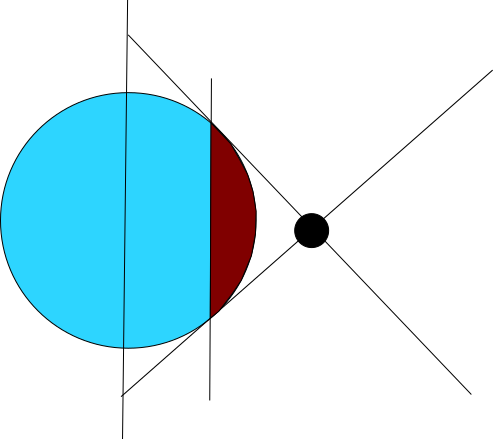
\includegraphics[width=0.4\textwidth]{img/fig31.png}
  \caption{Figura que explica el desarrollo necesario, donde desde la vista del satelite la parte roja es visible mientras la azul es tapada por el planeta.}
  \label{img:31}
\end{figure}

En este caso el satelite esta geoestacionario y por tanto su velocidad angular es la misma que la de la tierra (puesto que da una vuelta completa en el mismo tiempo que lo da el punto sobre el que esta). El semieje de su orbita es el mismo que el del planeta. Por ultimo, para determinar el area que puede ver el satelite dependemos de la distancia que tenga frente al suelo. En particular en nuestro modelo, el satelite podra observar todo aquello que no sea tapado por la propia tierra. Es decir que lo que nos interesa es encontrar la distancia que hay entre un punto cuya recta tangente pase por el punto en el que se encuentra el satelite y el medio de la circunferencia (para una explicación grafica vea la figura \ref{img:31}). Esto tiene como consecuencia que tenemos la condición: \[
m_{s-p} = \frac{d C}{dx} \implies -\frac{y}{h-x}=-\frac{x}{\sqrt{r^2-x^2} }
.\] 

Esto sale de despejar $y$ como:  \[
y = \sqrt{r^2 - x^2} 
.\] 

Con lo que podemos desarrollar: 
\begin{align*}
-\frac{y}{h-x}=-\frac{x}{\sqrt{r^2-x^2} }\\
\frac{y}{h-x}=\frac{x}{y}\\
y^2 = x\left( h-x \right) \\
r^2 - x^2 = xh - x^2\\
r^2 = xh \\
x = \frac{r^2}{h}
.\end{align*}

Por lo tanto esta distancia depende del radio del circulo y de la altura del satelite. Con esto podemos definir entonces el casco que va a ser observable desde el satelite con $y=R$ y $r-x = H$ y el área de este tipo de objetos es: \[
  \pi \left( R^2 + H^2 \right) = \pi\left( y^2 + H^2 \right) = \pi\left( r^2 - x^2 + r^2 - 2xr + x^2 \right) 
.\] y esto equivale a:
\begin{align*}
  \pi\left( 2r^2 - 2xr \right) &= 2\pi r \left( r - x \right)  \\
  &= 2\pi r \left( r - \frac{r^2}{h} \right)  \\
  &= 2\pi r^2 \left( 1 - \frac{r}{h} \right)
.\end{align*}

y entonces el porcentaje de lo que se puede ver es:
\begin{align*}
  &= \frac{2\pi r^2\left( 1 - \frac{r}{h} \right) }{4\pi r^2} \\
  &= \frac{1-\frac{r}{h}}{2}
.\end{align*}


\chapter{}

\section{Enunciado}

A partir del diámetro angular del Sol y la duración del periodo de orbital de la tierra (un año), determine la densidad media del Sol.

\section{Solución}

\begin{align*}
  r = a\tan\left( \beta \right) \\
  \frac{T^2}{a^{3}} = \frac{4\pi^2}{GM}\\
  \frac{T^2}{\frac{r^{3}}{u^{3}}} = \frac{4\pi^2}{GM}\\
  \frac{T^2}{4r^{3}}= \frac{\pi^2}{4^{3}GM}\\
  \frac{T^2}{\frac{4}{3}\pi r^{3}} = \frac{3\pi}{u^{3}GM}\\
  \frac{M}{\frac{4}{3}\pi r^{3}}=\frac{3\pi}{u^{3}G T^2}\\
  \rho = 1434 \frac{kg}{m^3}
.\end{align*}


\chapter{}

\section{Enunciado}

En un Universo hipotético solo existen dos rocas de $5$ kg de masa cada una. Cada una orbita a la otra a una distancia de $1$ metro.¿Cual es el periodo orbital de este sistema binario de rocas?

\section{Solución}

En este caso utilizaremos un desarrollo muy similar al usado en el libro \textit{Mecánica Clásica} que esta en bloqueneon. Suponga que llamaremos a estas dos rocas cuerpo $1$ y cuerpo $2$. En este universo unicamente existirian 2 fuerzas  $F_{12}$ y $F_{21}$ que son la fuerza que hace un cuerpo sobre el otro y al reves. Note que por $3$ ley de Newton sabemos que $F_{12}=-F_{21}$. Ademas, tenemos que \[
\mu = \frac{m_1m_2}{m_1+m_2} = \frac{25}{10} = 2.5
.\] donde $M=m_1+m_2$ y con esto reducimos (como en el capitulo previamente citado) el movimiento de estos dos cuerpos al movimiento de un cuerpo de masa $\mu$ que orbita otro de masa infinita. Con esto entonces queda \[
F = \mu a
.\] ahora bien,  $F$ en este caso es la fuerza que hace el cuerpo dos sobre el cuerpo 1 que como sabemos en este caso esa interacción se da por gravedad y en consecuencia consiste en
\begin{align*}
  F = G \frac{m_1m_2}{r^2}\\
  = G \frac{25 kg^2}{1 m^2}\\
  = G*25
.\end{align*}

Por tanto $a$ es $a = \frac{F}{\mu}$ lo cual entonces significa que:

\begin{align*}
  a = \frac{25G}{2.5}\\
  = \frac{25G}{\frac{25}{10}}\\
  = 10G
.\end{align*}

Por lo tanto, tenemos una aceleración constante. Sabemos ademas que ambas aceleraciónes son iguales pues las fuerzas son iguales y las masas tambien por lo tanto solo debemos resolver para una de las aceleraciones que es:
\begin{align*}
  a_1 = \frac{5}{10}10G = 5G
.\end{align*}

Dado que $G$ es una constante sabemos que la integral de esta aceleración para el movimiento seria la velocidad y dado que solo nos interesa la magnitud (y sabemos que es una aceleración centripeta) podemos usar: \[
a_1 = \frac{v^2}{r}
.\] en donde en este caso $r$ es $0.5 m$ dado que es el centro de masa (que esta en el centro por que trabajamos con masas iguales. Esto entonces queda:
\begin{align*}
  v_1 = \sqrt{a_1r} \\
  = \sqrt{5G*\frac{5}{10}} \\
  = \sqrt{\frac{25}{10}G}
.\end{align*}

Ahora bien, dado que tenemos esta velocidad (que es tangencial) podemos encontrar una velocidad angular simplemente dividiendo por $r$
\begin{align*}
  v_1 = \frac{\sqrt{\frac{25}{10}G} }{0.5}\\
  = \frac{5 \sqrt{\frac{G}{10}} }{\frac{5}{10}}\\
  = \sqrt{10G}
.\end{align*}

Por lo tanto lo unico que necesitamos es encontrar lo que se demora en dar una vuelta completa lo cual es:
\begin{align*}
  T = \frac{2\pi}{\sqrt{10G}}
.\end{align*}

\chapter{}
\section{Enunciado}

Resolver el problema $99$ del texto de \textit{Física General de Halliday \& Resnik}

\section{Solución}

\subsection{Parte A}

\begin{align*}
  U\left( x \right) &= -Gm \int \frac{1}{\sqrt{x^2+R^2} }dM\\
  &= - \frac{GmM}{\sqrt{x^2 + R^2} } \\
  &\implies ||F||= -\frac{dU}{dx}=+\frac{GmMx}{\left( x^2+R^2 \right)^{\frac{3}{2}}}
.\end{align*}

\subsection{Parte B}

\begin{align*}
  \Delta U &= U\left( 0 \right) - U\left( x \right)  \\
  &= -GmM \left( \frac{1}{R}-\frac{1}{\sqrt{x_4R^2} } \right)  \\
  \Delta E &\implies \Delta K = - \Delta U \\
  -\Delta U &= \frac{1}{2}mv^2 \\
  v &= \sqrt{\frac{-2\Delta U}{m}}  \\
  v &= \sqrt{2GM\left( \frac{1}{R} - \frac{1}{x^2+R^2} \right) }
.\end{align*}
 

\chapter{}

\section{Enunciado}

Resolver el problema $11$ del texto de \textit{Física General de Halliday \& Resnik}

\section{Solución}

Para poder solucionar este punto haremos uso de la ecuación \[
g = g_0 + \Omega^2 R \sin\theta
.\] Esta ecuación puede ser encontrada en el Taylor Capitulo 9. Ahora bien, dado que todos los planetas son iguales en tamaño y en masa entonces $g_0$ es el mismo para todos los planetas. Por lo tanto, la única diferencia es $\theta$. Tomando en cuenta esto, note que los puntos $b, d, f$ estan en los polos y por lo tanto  $\theta = 0$ para todos estos casos y por lo tanto $\sin\left( \theta \right) = 0$ y dado que todos los otros puntos están en el ecuador entonces $\theta = \frac{\pi}{2}$ lo cual nos deja con $\sin\left( \theta \right) = 1$ y por lo tanto solo se organizan en función de su velocidad angular lo que nos deja con:
\begin{align*}
  a > c > e > b \ge d \ge f
.\end{align*}

\chapter{}

\section{Enunciado}

Resolver el problema $6$ del texto de \textit{Física General de Halliday \& Resnik}

\section{Solución}

\subsection{Parte A}

Note que $a_g = \frac{GM}{r^2}$ 

Por lo tanto
\begin{align*}
  \frac{M_1}{R_4^2} = \frac{M_2}{R_4^2} &> \frac{M_3}{R_4^2} = \frac{M_4}{R_4^2}\\
  M_1 = M_2 &> M_3 = M_4
.\end{align*}

\subsection{Parte B}

Note que $R_1<R_2$ y $R_3<R_4$, entonces $\frac{1}{R_1}>\frac{1}{R_2}$ y $\frac{1}{R_3}>\frac{1}{R_4}$ Ademas note que $R_2=R_3$ y dado que $M_2>M_3$ entonces $\rho_2>\rho_3$ por lo que:
\begin{align*}
  \rho_1>\rho_2>\rho_3>\rho_4
.\end{align*}


\chapter{}

\section{Enunciado}

Calcular la dependencia del ángulo alpha con la latitud. Graficar alpha
versus la latitud geográfica (-90, 90). Interprete físicamente sus resultados.
Presente su discusión comentando lo que ocurre en cinco ciudades ubicadas en
latitudes que ayuden a la interpretación de sus resultados.

\section{Solución}

Quizás lo mas prudente para iniciar este punto es deducir la ecuación para $\alpha_{max}$

\begin{align*}
  F &= F_G + F_C \\
  m \ddot{r} &= - \frac{GM_{tierra} m}{R^2} \hat{r} + m \Omega^2 R \sin\theta \hat{p} \\
  \ddot{r} &= - \frac{GM_{Tierra}}{R^2} \hat{r} + \Omega^2 R\sin\theta \hat{p} 
.\end{align*}

Ahora con un dibujo expliquemos lo que pasa:

\begin{figure}[H]
  \centering
  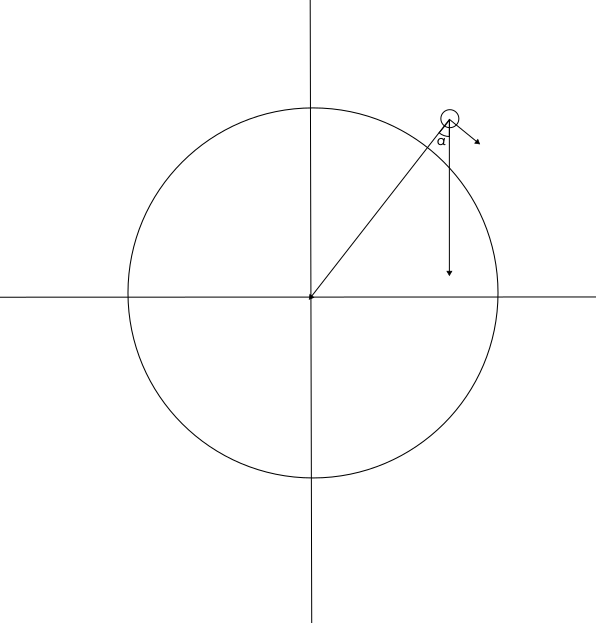
\includegraphics[width=0.4\textwidth]{img/fig91.png}
  \caption{Grafica en la que se muestra las distintas gravedades.}
  \label{fig:fig91}
\end{figure}

Con esta figura, podemos ver que $\alpha$ esta definido entre estas dos fuerzas. Con lo cual podemos deducir que $\tan(\alpha) = \frac{\left| g_{tan} \right| }{\left| g_{rad} \right| }$. Ademas, para $\alpha$ pequeño tenemos que $\tan\left( \alpha \right) = \alpha$ entonces de aqui podemos deducir que:
\begin{align*}
  \alpha &= \frac{\Omega^2 R \sin\left( \theta \right) \cos\left( \theta \right) }{g_0 - \Omega^2 R \sin^2\left( \theta \right) }
.\end{align*}

Con esto solucionado podemos simplemente programar las pruebas y la solución de la siguiente manera:

\lstinputlisting[language=Python]{code/graficas.py}

Lo cual nos da el siguiente resultado:
\begin{figure}[H]
  \centering
  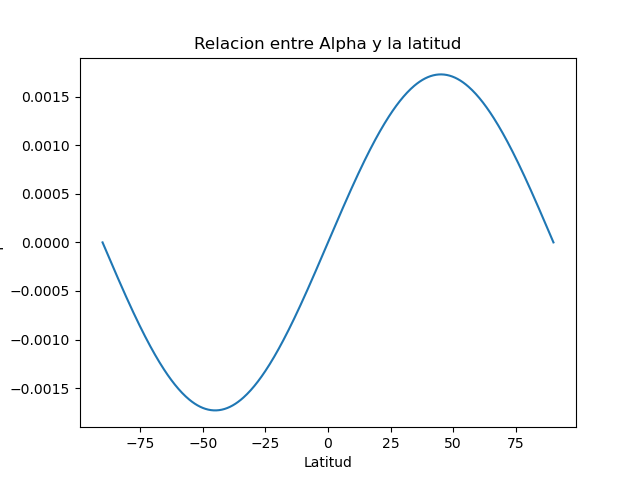
\includegraphics[width=0.8\textwidth]{img/alpha_tierra.png}
  \caption{Imagen del $\alpha$ maximo segun el angulo}
  \label{fig:img-alpha_tierra-png}
\end{figure}



\chapter{}

En este caso, lo mas simple es trabajarlo por medio de un codigo. A continuación se encuentra ese codigo

\lstinputlisting[language=Python]{code/main.py}

\begin{table}[htpb]
  \centering
  \caption{Tabla con los resultados}
  \label{tab:label}
  \begin{tabular}{llrrrrr}
    \hline
 & Cuerpo Celeste & $R (m)$ & $T (s)$ & $g (\frac{m}{s^2})$ & $\omega (\frac{rad}{s})$ & $\alpha_{max} (rad)$ \\
 \hline
    0 & Sol & 696000000.000000 & 2140000.000000 & 274.000000 & 0.000003 & 0.000022 \\
    1 & Júpiter & 69900000.000000 & 35800.000000 & 24.790000 & 0.000176 & 0.086637 \\
    2 & Tierra & 6370000.000000 & 86400.000000 & 9.810000 & 0.000073 & 0.003434 \\
    3 & Marte & 3390000.000000 & 88700.000000 & 3.720000 & 0.000071 & 0.004573 \\
    4 & Luna & 1740000.000000 & 2360000.000000 & 1.620000 & 0.000003 & 0.000008 \\
    5 & Estrella de neutrones & 10000.000000 & 0.001000 & 1000000000000.000000 & 6283.185307 & 0.376002 \\
    \hline
  \end{tabular}
\end{table}


\end{document}
